\documentclass[trans,aspectratio=169]{beamer}

\usepackage{etex}
\usepackage{amsthm}
\usepackage{xcolor}
\usepackage{wrapfig}
\usepackage{soul}
\usepackage{lipsum}
\usepackage{booktabs}
\usepackage{graphicx}
\usepackage{algorithm}
\usepackage{algorithmic}
\usepackage{answers}
\usepackage[absolute,overlay]{textpos}
\usepackage{verbatim}
\usepackage{fancyvrb}
\usepackage{xspace}
%\usepackage[labelsep=none]{caption}
\usepackage{tikz}
\usepackage{units}
\usepackage{makeidx}
\usepackage{tabularx}
\usepackage{colortbl}
\usepackage{multirow}
\usepackage{calc}
%\usepackage{graphicx}
%\usepackage{array}
%\usepackage[all]{xy}
%%\usepackage{theapa}
%\usepackage{tikz}
%\usetikzlibrary{shapes.geometric} 
%\usetikzlibrary{shadows} 
%\usetikzlibrary{positioning}
%\usepackage{algorithm}
%%\usepackage{algorithmic}
%\usepackage{algorithmic}
%%\usepackage{algpseudocode}
%\usepackage{natbib}
%\usepackage{apalike}
\usepackage{../book/haldefs}

\mode<presentation>
{
%  \usetheme{AnnArbor}
%  \usetheme{Antibes}
%  \usetheme{Bergen}
%  \usetheme{Berkeley}
%  \usetheme{Berlin}
%  \usetheme{Boadilla}
%  \usetheme{boxes}
%  \usetheme{CambridgeUS}
%  \usetheme{Copenhagen}
%  \usetheme{Darmstadt}
%  \usetheme{default}
%  \usetheme{Dresden}
%  \usetheme{Frankfurt}
%  \usetheme{Goettingen}
%  \usetheme{Hannover}
%  \usetheme{Ilmenau}
%  \usetheme{JuanLesPins}
%  \usetheme{Luebeck}
%  \usetheme{Madrid}
%  \usetheme{Malmoe}
%  \usetheme{Marburg}
%  \usetheme{Montpellier}
%  \usetheme{PaloAlto}
%  \usetheme{Pittsburgh}
%  \usetheme{Rochester}
%  \usetheme{Singapore}
%  \usetheme{Szeged}
%  \usetheme{Warsaw}
  \usetheme{Unife}

%\usecolortheme{lily}% 
  % or ...

  \setbeamercovered{transparent}
  % or whatever (possibly just delete it)
}


\usepackage[english]{babel}
% or whatever

%\usepackage[latin1]{inputenc}
% or whatever
\usetikzlibrary{shapes,snakes}
%%% Local Variables: 
%%% mode: latex
%%% TeX-master: "courseml"
%%% End: 

%%%%%%%%%%% COLORS

\definecolor{darkgrey}{rgb}{0.2,0.2,0.2}
\definecolor{grey}{rgb}{0.9,0.9,0.9}
\definecolor{darkblue}{rgb}{0.0,0.0,0.5}
\definecolor{darkpurple}{rgb}{0.4,0.0,0.4}
\definecolor{darkred}{rgb}{0.5,0.0,0.0}
\definecolor{darkorange}{rgb}{0.5,0.45,0.4}
\definecolor{darkgreen}{rgb}{0.0,0.5,0.0}
\definecolor{darkergreen}{rgb}{0.0,0.4,0.0}
\definecolor{lightblue}{rgb}{0.8,0.8,1.0}
\definecolor{lightgreen}{rgb}{0.8,1.0,0.8}
\definecolor{lightred}{rgb}{1.0,0.8,0.8}
\definecolor{lightyellow}{rgb}{1.0,1.0,0.8}
\definecolor{lightorange}{rgb}{1.0,0.9,0.8}
\definecolor{lightgrey}{rgb}{0.96,0.97,0.98}
\definecolor{Sepia}{HTML}{671800}

%%%%%%%%%%%%% FORMATTING
%
%\newcommand*\chapterlabel{}
%\makeatletter
%\titleformat{\chapter}%
%  [block]                                % shape
%  {\gdef\chapterlabel{}
%   \normalfont\sffamily\Huge\bfseries\scshape}            % format applied to label+text
%  {\gdef\chapterlabel{\thechapter~|~}}    % 
%  {0pt}                                  % horizontal separation between label and title body
%  {\begin{tikzpicture}[remember picture,overlay]
%    \node[yshift=-3cm] at (current page.north west)
%      {\begin{tikzpicture}[remember picture, overlay]
%        \draw[fill=lightgreen] (0,0) rectangle
%          (\paperwidth,3cm);
%        \node[anchor=east,xshift=.9\paperwidth,rectangle,
%              rounded corners=20pt,inner sep=11pt,
%              fill=darkergreen]
%              {\color{white}\chapterlabel#1};
%       \end{tikzpicture}
%      };
%   \end{tikzpicture}
%  }% before the title body
%  []%after the title body
%\makeatother 
%%\titlespacing*{\chapter}{0pt}{50pt}{-10pt}
%
%\newcommand{\sectionsize}{}
%\titleformat{\section}%
%  [hang]% shape
%  {\normalfont\Large\itshape}% format applied to label+text
%  {\textcolor{darkergreen}{\makebox[0pt][r]{\thesection\quad }#1}}% label
%  {1em}% horizontal separation between label and title body
%  {}% before the title body
%  []% after the title body
%
%\titleformat{\subsection}%
%  [hang]% shape
%  {\normalfont\large\itshape}% format applied to label+text
%  {\textcolor{darkergreen}{\makebox[0pt][r]{\thesubsection\quad }#1}}% label
%  {1em}% horizontal separation between label and title body
%  {}% before the title body
%  []% after the title body



%%%%%%%%%%% EXERCISE STUFF

\newtheorem{Ex}{Exercise}
\newenvironment{exercises}{\section{Exercises}}{}
% \center\begin{tabular}{c}\hline{\bf\Large Exercises}\\\hline\end{tabular}}{}

%\Newassociation{solution}{Soln}{solutions}
%\Newassociation{hint}{Hint}{solutions}
\newcommand{\prehint}{~[Hint]}
\newcommand{\presolution}{}
\newcommand{\Opensolutionshook}[2]%
  {\Writetofile{#1}{}}
%\renewcommand{\Solnlabel}[1]{%
%  {\Large\linespread{1}%
%  \begin{tabular}{|p{\textwidth}@{}|}%
%    \hline%
%    \emph{Solution #1}\\%
%    \hline%
%  \end{tabular}\newline}}
%\renewcommand{\Hintlabel}[1]{\emph{Hint #1}}


\newcommand{\emptylist}{[ ]}
\newcommand{\pushlist}[1]{{\ensuremath \oplus} #1}

\newcommand*\learningproblemargument{}
\newsavebox{\learningproblembox}
\newenvironment{learningproblemenv}[1]
  {\gdef\learningproblemargument{#1}\begin{lrbox}{\learningproblembox}\begin{minipage}{4in}}
  {\end{minipage}\end{lrbox}%
   \tikzstyle{mybox} = [draw=darkgreen, fill=green!5, very thick, rectangle, rounded corners, inner sep=10pt, inner ysep=12pt]%
   \tikzstyle{fancytitle} =[fill=darkgreen, text=white, rectangle, rounded corners]%
   \vspace{1em}
   \noindent
   \begin{tikzpicture}
     \node [mybox] (box) {\usebox{\learningproblembox}};
     \node [fancytitle, right=10pt] at (box.north west) {\normalfont\sffamily\Large\bfseries\scshape Task: \learningproblemargument};
   \end{tikzpicture}
  }

\newcommand{\learningproblem}[3]{
  \begin{learningproblemenv}{#1}
    \emph{Given:}
    \begin{enumerate}
      #2
    \end{enumerate}
    \emph{Compute:} #3
  \end{learningproblemenv}}

\newcommand{\lprob}[1]{{\normalfont\sffamily\scshape #1}}

%%%%%%%%%%% ENVIRONMENTS

\DefineVerbatimEnvironment%
  {chapternotes}{Verbatim}
  {baselinestretch=1.0,frame=single,fillcolor=\color{lightgreen}}
%\renewenvironment{chapternotes}{\begin{comment}}{\end{comment}}

\newenvironment{editedout}{\begin{comment}}{\end{comment}}

\newenvironment{derivation}
  {\begin{eqnarray}}
  {\end{eqnarray}}

\newcommand{\derivstep}[2]{#1\sidenote{#2}}

%\makeatletter\newenvironment{learninggoals}{%
%   ~\\\noindent\begin{lrbox}{\@tempboxa}\begin{shadowblock}{\columnwidth}\begin{itemize}}{\end{itemize}\end{shadowblock}\end{lrbox}%
%   {\usebox{\@tempboxa}}
%}\makeatother

%\newenvironment{learningobjectives}
%  {\begin{marginfigure}\begin{learninggoals}\item[]\item[] \hspace{-2em} {\bf Learning Objectives:}}
%  {\end{learninggoals}\end{marginfigure}}

\newsavebox{\objectivesbox}
\newlength{\objectivesheight}
\newenvironment{learningobjectives}
  {\begin{lrbox}{\objectivesbox}\begin{minipage}{2in}\vspace{2pt}{\bf Learning Objectives:}\begin{footnotesize}\begin{itemize}}
  {\end{itemize}\end{footnotesize}\end{minipage}\end{lrbox}\begin{textblock}{2}(10.2,2.5)\begin{shadowblock}{2in}\usebox{\objectivesbox}\end{shadowblock}\end{textblock}\settoheight{\objectivesheight}{\usebox{\objectivesbox}}}

\newenvironment{chapterintro}
  {}
  {}

\newcommand*\vignetteargument{}
\newsavebox{\vignettebox}
\newenvironment{vignette}[1]
  {\gdef\vignetteargument{#1}\begin{lrbox}{\vignettebox}\begin{minipage}{6.4in}}
  {\end{minipage}\end{lrbox}%
   \tikzstyle{mybox} = [draw=Periwinkle, fill=Periwinkle!5, very thick, rectangle, rounded corners, inner sep=10pt, inner ysep=12pt]%
   \tikzstyle{fancytitle} =[fill=Periwinkle, text=white, rectangle, rounded corners]%
   \vspace{1em}
   \noindent
   \begin{tikzpicture}
     \node [mybox] (box) {\usebox{\vignettebox}};
     \node [fancytitle, right=10pt] at (box.north west) {\normalfont\sffamily\Large\bfseries\scshape Vignette: \vignetteargument};
   \end{tikzpicture}
  }

%[transform shape, baseline=-3.5cm]
\newcommand*\mathreviewargument{}
\newsavebox{\mathreviewbox}
\newenvironment{mathreview}[1]
  {\gdef\mathreviewargument{#1}\begin{lrbox}{\mathreviewbox}\begin{minipage}{6.4in}}
  {\end{minipage}\end{lrbox}%
   \tikzstyle{mybox} = [draw=Sepia, fill=Sepia!5, very thick, rectangle, rounded corners, inner sep=10pt, inner ysep=12pt]%
   \tikzstyle{fancytitle} =[fill=Sepia, text=white, rectangle, rounded corners]%
   \begin{figure*}[t]
     \begin{tikzpicture}
       \node [mybox] (box) {\usebox{\mathreviewbox}};
       \node [fancytitle, right=10pt] at (box.north west) {\normalfont\sffamily\Large\bfseries\scshape Math Review | \mathreviewargument};
     \end{tikzpicture}
     \caption[Math Review: \mathreviewargument]{~}
   \end{figure*}%
  }


%\newenvironment{chapterquote}
%  {\textblockcolor{grey}\begin{textblock}{6.5}(8,1)}
%  {\end{textblock}}

%\newenvironment{chapterimage}
%  {\textblockcolor{white}\begin{textblock}{6.5}(8,1)}
%  {\end{textblock}}


%  {\par\linespread{1}\center%
%   \begin{greybox}%
%   \begin{tabular}{|p{4in}|}%
%     \hline\vspace{+0.02in}%
%     \rule{1ex}{1ex} Learning Goals \rule{1ex}{1ex}%
%     }
%  { \vspace{+0.05in}\\\hline%
%   \end{tabular}\vspace{+0.1in}\end{greybox}\\}\makeatother


%%%%%%%%%%% COMMANDS

\newcommand{\bigemph}[1]{\textcolor{darkblue}{\bf #1}}

\newcommand{\dependencies}[1]{\marginnote[2.5in]{Dependencies: #1}}

%\newcommand{\dependencies}[1]{\begin{textblock}{2}(10.2,2.5)Dependencies: #1\end{textblock}}

%\sethlcolor{lightyellow}

\newcommand{\concept}[1]{\hl{\bf #1}\index{#1}}
\newcommand{\koncept}[2]{\hl{\bf #1}\index{#2}}

\newcommand{\chref}[1]{Chapter~\ref{#1}}


\newcommand{\chapterquote}[2]
  {\tikzstyle{mybox} = [draw=darkergreen, fill=green!20, very thick, rectangle, rounded corners, inner sep=5pt, inner ysep=5pt]
   \tikzstyle{fancytitle} =[fill=darkergreen, text=white]
   \begin{textblock}{7.5}(2,2.5)
   \begin{tikzpicture}[transform shape, rotate=0, baseline=-3.5cm]
   \noindent%
   \node [mybox] (box) {%
    \begin{minipage}[t!]{\textwidth}
      \noindent%
      \begin{large}%
      \textsf{#1}%
      \end{large}
      \hfill\textcolor{darkergreen}{\textsf{--~#2}}
    \end{minipage}
    };
%   \node[fancytitle] at (box.south) {\emph{-- #2}};
  \end{tikzpicture}
  \end{textblock}}

\newcommand{\chapterimage}[2]
  {\tikzstyle{mybox} = [draw=darkergreen, fill=green!20, very thick, rectangle, rounded corners, inner sep=5pt, inner ysep=5pt]
   \tikzstyle{fancytitle} =[fill=darkergreen, text=white]
   \begin{textblock}{7.5}(2,2.5)
   \begin{tikzpicture}[transform shape, rotate=0, baseline=-3.5cm]
   \noindent
   \node [mybox] (box) {%
    \begin{minipage}[t!]{\textwidth}
      \includegraphics[width=\textwidth]{#1}

      \hfill\textcolor{darkergreen}{\textsf{--~#2}}
    \end{minipage}
    };
%   \node[fancytitle] at (box.south) {\emph{-- #2}};
  \end{tikzpicture}
  \end{textblock}}

\newcommand{\chapterimageopt}[3]
  {\tikzstyle{mybox} = [draw=darkergreen, fill=green!20, very thick, rectangle, rounded corners, inner sep=5pt, inner ysep=5pt]
   \tikzstyle{fancytitle} =[fill=darkergreen, text=white]
   \begin{textblock}{7.5}(2,2.5)
   \begin{tikzpicture}[transform shape, rotate=0, baseline=-3.5cm]
   \noindent
   \node [mybox] (box) {%
    \begin{minipage}[t!]{\textwidth}
      \includegraphics[#2]{#1}

      \hfill\textcolor{darkergreen}{\textsf{--~#3}}
    \end{minipage}
    };
%   \node[fancytitle] at (box.south) {\emph{-- #2}};
  \end{tikzpicture}
  \end{textblock}}


\newcommand{\monthyear}{%
  \ifcase\month\or January\or February\or March\or April\or May\or June\or
  July\or August\or September\or October\or November\or
  December\fi\space\number\year
}

\newcommand{\blankpage}{\newpage\hbox{}\thispagestyle{empty}\newpage}
\newcommand{\mycite}[1]{\ e{\citealt{#1}}}
\newcommand{\bookurl}{\url{http://hal3.name/courseml/}}

\newcommand{\TODOFigure}[2]{%
  \begin{marginfigure}
    \framebox[\textwidth][c]{\begin{minipage}{\textwidth}\rule{0pt}{2in}\end{minipage}}
    \caption{{\tt #1}: #2}
    \label{fig:#1}
  \end{marginfigure}}

\newlength{\NextFigureOffset}
\newcommand{\ResetNextFigure}{\setlength{\NextFigureOffset}{0mm}}
\newcommand{\MoveNextFigure}[1]{\setlength{\NextFigureOffset}{#1}}

\ResetNextFigure{}

\newcommand{\Figure}[2]{%
  \begin{marginfigure}[\NextFigureOffset]
    \begin{centering}
    \includegraphics[width=\textwidth]{figs/#1}
    \caption{#2}
    \label{fig:#1}
    \end{centering}
  \end{marginfigure}
  \ResetNextFigure{}
  }

\newcommand{\Table}[4]{%
  \begin{margintable}
    \begin{centering}
    \begin{tabular}{#3}
      #4
    \end{tabular}
    \caption{#2}
    \label{tab:#1}
    \end{centering}
  \end{margintable}}

\newcommand{\TableSize}[5]{%
  \begin{margintable}
    \begin{centering}
    \begin{#1}
    \begin{tabular}{#4}
      #5
    \end{tabular}
    \caption{#3}
    \label{tab:#2}
    \end{#1}
    \end{centering}
  \end{margintable}}

\newcommand{\thinkaboutit}[1]{%
\marginnote{
   \noindent
  \begin{tikzpicture}[transform shape, rotate=0, baseline=-3.5cm]
   \node [draw=Blue, fill=Blue!10, very thick, rectangle, rounded corners, inner sep=8pt, inner ysep=5pt] (box) {%
    \begin{minipage}[t!]{1.8in}
      #1
    \end{minipage}
    };
   \node[fill=Blue, text=white] at (box.west) {\textsf{\LARGE ?}};
  \end{tikzpicture}
}
}

\newenvironment{myproof}[1]%
  {\begin{proof}[Proof of Theorem~#1]}
  {\end{proof}}

\definecolor{gray0.00}{rgb}{1,1,1}
\definecolor{gray0.20}{rgb}{0.9,0.9,0.9}
\definecolor{gray0.26}{rgb}{0.87,0.87,0.87}
\definecolor{gray0.30}{rgb}{0.85,0.85,0.85}
\definecolor{gray0.32}{rgb}{0.84,0.84,0.84}
\definecolor{gray0.33}{rgb}{0.835,0.835,0.835}
\definecolor{gray0.40}{rgb}{0.8,0.8,0.8}
\definecolor{gray0.48}{rgb}{0.76,0.76,0.76}
\definecolor{gray0.53}{rgb}{0.735,0.735,0.735}
\definecolor{gray0.57}{rgb}{0.715,0.715,0.715}
\definecolor{gray0.60}{rgb}{0.7,0.7,0.7}
\definecolor{gray0.68}{rgb}{0.66,0.66,0.66}
\definecolor{gray0.74}{rgb}{0.63,0.63,0.63}
\definecolor{gray0.80}{rgb}{0.6,0.6,0.6}
\definecolor{gray0.88}{rgb}{0.56,0.56,0.56}
\definecolor{gray1.00}{rgb}{0.5,0.5,0.5}
\newcommand{\showfscore}[1]{\cellcolor{gray#1}{#1}}

\renewcommand{\vx}{{\vec x}}
\renewcommand{\vw}{{\vec w}}
\renewcommand{\vg}{{\vec g}}
\renewcommand{\vz}{{\vec z}}
\renewcommand{\vth}{{\vec \theta}}
\renewcommand{\dotp}[2]{#1 \cdot #2}

\renewcommand{\txtif}{\text{if } }

\renewcommand{\ones}{\ensuremath{\mathbf{1}}}
\renewcommand{\zeros}{\ensuremath{\mathbf{0}}}
\renewcommand{\eye}{\ensuremath{\mathbf{I}}}

%\let\Oldtimes\times
%\renewcommand{\times}{\!\!\Oldtimes\!\!}

\renewcommand{\myiff}{\Longleftrightarrow}

\renewcommand{\subgrad}{\pmb\partial}

\renewcommand{\partialby}[1]{\frac \partial {\partial #1}}
\renewcommand{\partialof}[2]{\frac {\partial #1} {\partial #2}}

\renewcommand{\xth}[1]{{}^{\textcolor{darkgrey}{\textsf{(#1)}}}}
\renewcommand{\kth}{\xth{k}}
\renewcommand{\Kth}{\xth{K}}
\renewcommand{\kpth}{\xth{k-1}}
\renewcommand{\zth}{\xth{0}}
\renewcommand{\oth}{\xth{1}}
\newcommand{\newth}{\xth{new}}

\renewcommand{\pth}{p_{\vec\th}}

\newcommand{\becauseof}[1]{&&& \textsf{\textcolor{darkred}{#1}}}

% ALGORITHMIC STUFF

\algsetup{linenosize=\tiny,
          linenodelimiter=:
          }

\renewcommand{\algorithmicfont}{\normalfont\sffamily\normalsize\bfseries}
\newcommand{\algorithmiccolor}{darkpurple}

\newcommand{\GOTO}[1]{\STATE
  \textcolor{\algorithmiccolor}{\algorithmicfont goto~} {\large #1}}

\renewcommand{\algorithmicif}{\textcolor{\algorithmiccolor}{\algorithmicfont if}}
\renewcommand{\algorithmicrequire}{\textcolor{\algorithmiccolor}{\algorithmicfont Require:}}
\renewcommand{\algorithmicensure}{\textcolor{\algorithmiccolor}{\algorithmicfont Ensure:}}
\renewcommand{\algorithmicend}{\textcolor{\algorithmiccolor}{\algorithmicfont end}}
\renewcommand{\algorithmicif}{\textcolor{\algorithmiccolor}{\algorithmicfont if}}
\renewcommand{\algorithmicthen}{\textcolor{\algorithmiccolor}{\algorithmicfont then}}
\renewcommand{\algorithmicelse}{\textcolor{\algorithmiccolor}{\algorithmicfont else}}
\renewcommand{\algorithmicelsif}{\algorithmicelse\ \algorithmicif}
\renewcommand{\algorithmicendif}{\algorithmicend\ \algorithmicif}
\renewcommand{\algorithmicfor}{\textcolor{\algorithmiccolor}{\algorithmicfont for}}
\renewcommand{\algorithmicforall}{\textcolor{\algorithmiccolor}{\algorithmicfont for all}}
\renewcommand{\algorithmicdo}{\textcolor{\algorithmiccolor}{\algorithmicfont do}}
\renewcommand{\algorithmicto}{\textcolor{\algorithmiccolor}{\algorithmicfont to}}
\renewcommand{\algorithmicendfor}{\algorithmicend\ \algorithmicfor}
\renewcommand{\algorithmicwhile}{\textcolor{\algorithmiccolor}{\algorithmicfont while}}
\renewcommand{\algorithmicendwhile}{\algorithmicend\ \algorithmicwhile}
\renewcommand{\algorithmicloop}{\textcolor{\algorithmiccolor}{\algorithmicfont loop}}
\renewcommand{\algorithmicendloop}{\algorithmicend\ \algorithmicloop}
\renewcommand{\algorithmicrepeat}{\textcolor{\algorithmiccolor}{\algorithmicfont repeat}}
\renewcommand{\algorithmicuntil}{\textcolor{\algorithmiccolor}{\algorithmicfont until}}
\renewcommand{\algorithmicprint}{\textcolor{\algorithmiccolor}{\algorithmicfont print}}
\renewcommand{\algorithmicreturn}{\textcolor{\algorithmiccolor}{\algorithmicfont return}}
\renewcommand{\algorithmictrue}{\textcolor{\algorithmiccolor}{\algorithmicfont true}}
\renewcommand{\algorithmicfalse}{\textcolor{\algorithmiccolor}{\algorithmicfont false}}
\renewcommand{\algorithmicand}{\textcolor{\algorithmiccolor}{\algorithmicfont and}}
\renewcommand{\algorithmicor}{\textcolor{\algorithmiccolor}{\algorithmicfont or}}

\renewcommand{\algorithmiccomment}[1]{\hfill\textcolor{Sepia}{\normalfont\sffamily// #1}}

\newcommand{\VAR}[1]{\textcolor{darkblue}{\textit{#1}}}
\newcommand{\CON}[1]{\textcolor{darkgrey}{\textit{#1}}}
\newcommand{\FUN}[1]{\textcolor{blue}{\textsc{#1}}}
\newcommand{\STR}[1]{\textcolor{darkergreen}{\textsc{#1}}}
\newcommand{\VARm}[1]{\textcolor{darkblue}{\ensuremath #1}}
\newcommand{\FUNm}[1]{\textcolor{blue}{\ensuremath #1}}

\newcommand{\SETST}[1]{\STATE \VAR{#1} $\leftarrow$ }
\newcommand{\SAMPLE}[1]{\STATE \VAR{#1} $\sim$ }

\newcommand{\feat}[1]{\textsc{\textcolor{darkpurple}{#1}}}

\floatname{algorithm}{\textcolor{\algorithmiccolor}{\algorithmicfont Algorithm}}

%\newcommand{\newalgorithm}[3]{%
%  \begin{algorithm}[t]
%    \label{alg:#1}
%    \caption{#2}
%    \begin{small}
%      \begin{algorithmic}[1]
%        #3
%      \end{algorithmic}
%    \end{small}
%  \end{algorithm}}
\newcommand{\newalgorithm}[3]{%
    \begin{small}
      #2
      \begin{algorithmic}[1]
        #3
      \end{algorithmic}
    \end{small}
}

\newcommand{\categ}[1]{\textsc{\textcolor{darkgrey}{#1}}}

%%%%%%%%%%%% TIKZ STUFF

%
% Boxed environment with semi-transparent shadow.
%
\newlength{\boxw}
\newlength{\boxh}
\newlength{\shadowsize}
\newlength{\boxroundness}
\newlength{\tmpa}
\newsavebox{\shadowblockbox}

\setlength{\shadowsize}{6pt}
\setlength{\boxroundness}{3pt}

\newenvironment{mycomment}{\begin{comment}}{\end{comment}}

\newenvironment{shadowblock}[1]%
{\begin{lrbox}{\shadowblockbox}\begin{minipage}{#1}}%
{\end{minipage}\end{lrbox}%
\settowidth{\boxw}{\usebox{\shadowblockbox}}%
\settodepth{\tmpa}{\usebox{\shadowblockbox}}%
\settoheight{\boxh}{\usebox{\shadowblockbox}}%
\addtolength{\boxh}{\tmpa}%
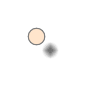
\begin{tikzpicture}
    \addtolength{\boxw}{\boxroundness * 2}
    \addtolength{\boxh}{\boxroundness * 2}

    \foreach \x in {0,.05,...,1}
    {
        \setlength{\tmpa}{\shadowsize * \real{\x}}
        \fill[xshift=\shadowsize - 1pt,yshift=-\shadowsize + 1pt,
                black,opacity=.04,rounded corners=\boxroundness]
            (\tmpa, \tmpa) rectangle +(\boxw - \tmpa - \tmpa,
                \boxh - \tmpa - \tmpa);
    }

    \filldraw[fill=lightorange, draw=black!50, rounded corners=\boxroundness]
        (0, 0) rectangle (\boxw, \boxh);
    \draw node[xshift=\boxroundness,yshift=\boxroundness,
        inner sep=1pt,outer sep=1pt,anchor=south west]
             (0,0) {\usebox{\shadowblockbox}};
\end{tikzpicture}}


%%%%%%%%5

\newcommand{\ceil}[1]{\left\lceil{#1}\right\rceil}

\newcommand{\optimize}[4]{%
  \begin{align}
    \min_{\substack{#2}}\quad & \label{opt:#1} #3 \\
    \text{subj. to}\quad & \nonumber #4
  \end{align}}

\newcommand{\optimizeoneline}[4]{%
  \begin{align}
    \min_{\substack{#2}}\quad & \label{opt:#1} #3 \quad
    \text{subj. to}\quad #4
  \end{align}}

\newcommand{\optimizemax}[4]{%
  \begin{align}
    \max_{\substack{#2}}\quad & \label{opt:#1} #3 \\
    \text{subj. to}\quad & \nonumber #4
  \end{align}}

\newcommand{\optimizemaxoneline}[4]{%
  \begin{align}
    \max_{\substack{#2}}\quad & \label{opt:#1} #3 \quad
    \text{subj. to}\quad #4
  \end{align}}

\newcommand{\optimizeuc}[3]{%
  \begin{align}
    \min_{\substack{#2}}\quad & \label{opt:#1} #3
  \end{align}}

\newcommand{\optimizeLagrange}[4]{%
  \begin{align}
    \max_{\substack{#2}} \min_{\substack{#3}}\quad & \label{opt:#1} #4
  \end{align}}

\newcommand{\optimizemaxuc}[3]{%
  \begin{align}
    \max_{\substack{#2}}\quad & \label{opt:#1} #3
  \end{align}}

\newcommand{\optimizemaxLagrange}[4]{%
  \begin{align}
    \min_{\substack{#2}} \max_{\substack{#3}}\quad & \label{opt:#1} #4
  \end{align}}

%\newtheorem{theorem}{Theorem}
%\newtheorem{definition}{Definitions}

%%% Local Variables: 
%%% mode: latex
%%% TeX-master: "courseml"
%%% End: 



% Or whatever. Note that the encoding and the font should match. If T1
% does not look nice, try deleting the line with the fontenc.
\newcommand{\myalert}[1]{{%\color{red}
 #1}}
\iffalse
\begin{learningobjectives}
\item Describe the biological motivation behind the perceptron.
\item Classify learning algorithms based on whether they are
  error-driven or not.
\item Implement the perceptron algorithm for binary classification.
\item Draw perceptron weight vectors and the corresponding decision
  boundaries in two dimensions.
%\item Define linear separability, and be able to turn any arbitrary
%  data set into a linearly separable data set.
\item Contrast the decision boundaries of decision trees, nearest
  neighbor algorithms and perceptrons.
\item Compute the margin of a given weight vector on a given data set.
\end{learningobjectives}

\dependencies{\chref{sec:dt}, \chref{sec:knn}}

\newthought{So far, you've seen two types} of learning models: in
decision trees, only a small number of features are used to make
decisions; in nearest neighbor algorithms, all features are used
equally.  Neither of these extremes is always desirable.  In some
problems, we might want to use most of the features, but use some more
than others.

In this chapter, we'll discuss the \concept{perceptron} algorithm for
learning \concept{weights} for features.  As we'll see, learning
weights for features amounts to learning a \concept{hyperplane}
classifier: that is, basically a division of space into two halves by
a straight line, where one half is ``positive'' and one half is
``negative.''  In this sense, the perceptron can be seen as explicitly
finding a good \concept{linear decision boundary}.
\fi
\title[Perceptron]
{Perceptron}


\institute[] % (optional, but mostly needed)
{
%ENDIF -- University of Ferrara,  Italy\\
% fabrizio.riguzzi@unife.it
}
% - Use the \inst command only if there are several affiliations.
% - Keep it simple, no one is interested in your street address.
\date{}

\begin{document}
\begin{frame}
\titlepage 
\vspace{-2cm}
\begin{center}
Chapter 3 of ``A Course in  Machine Learning'' by Hal Daum\'e III

\url{http://ciml.info}

Conversion to beamer by Fabrizio Riguzzi
\end{center}

\end{frame}
  \renewcommand{\concept}[1]{\myalert{#1}}
  \renewcommand{\koncept}[2]{\myalert{#1}}

\renewcommand{\Figure}[3]{%
    \begin{center}
    \includegraphics[width=#3\textwidth]{../book/figs/#1}
    \end{center}
  }
  
\begin{frame}
  \frametitle{Bio-inspired Learning}
\begin{itemize}
\item Folk biology tells us that our brains are made up of a bunch of little
units, called \concept{neurons}, that send electrical signals to one
another.  
\item The \emph{rate} of firing tells us how ``activated'' a
neuron is. 
\item  A single neuron (see next slide) might have three incoming neurons. 
\item These
incoming neurons are firing at different rates (i.e., have different
\concept{activations}). 
\item Based on how much these incoming neurons are
firing, and how ``strong'' the neural connections are, our main neuron
will ``decide'' how strongly it wants to fire.
\item   And so on through the
whole brain. 
\item Learning in the brain happens by neurons becomming
connected to other neurons, and the strengths of connections adapting
over time.
\end{itemize}
\end{frame}

\begin{frame}
\frametitle{A picture of a neuron}
\Figure{perc:neuron}{a picture of a neuron}{0.45}
\end{frame}

\begin{frame}
  \frametitle{Bio-inspired Learning}
\begin{itemize}
\item The real biological world is much more complicated than this.
\item However, our goal isn't to build a brain, but to simply be
\emph{inspired} by how they work. 
\item We are going to think of our
classifier as a \emph{single} neuron. 
\item It receives input from
$D$-many other neurons, one for each input feature.  
\item The strength of
these inputs are the feature values.  
\item Each incoming connection has a weight
and the neuron simply sums up all the weighted inputs.
\item  Based on this
sum, it decides whether to ``fire'' or not.
\end{itemize}
\end{frame}
\begin{frame}
  \frametitle{Bio-inspired Learning}
\begin{itemize}
\item  Firing is interpreted as
being a positive example and not firing is interpreted as being a
negative example. 
\item If the weighted sum is positive, it
``fires'' and otherwise it doesn't fire.
\end{itemize}
\Figure{perc:example}{figure showing feature vector and weight
  vector and products and sum}{0.35}
\end{frame}
\begin{frame}
  \frametitle{Bio-inspired Learning}
\begin{itemize}
\item
Mathematically, an input vector $\vx = \langle x_1, x_2, \dots, x_D
\rangle\in \R^D$ arrives. 
\item The neuron stores $D$-many weights, $w_1, w_2,
\dots, w_D$.  
\item The neuron computes the sum:
\begin{equation} \label{eq:perc:sum}
a = \sum_{d=1}^D w_d x_d
\end{equation}
to determine its amount of ``activation.''
\item  If this activation is
positive (i.e., $a > 0$) it predicts that this example is a positive
example.  Otherwise it predicts a negative example.
\end{itemize}
\end{frame}

\begin{frame}
  \frametitle{Bio-inspired Learning}
\begin{itemize}
\item The prediction is $\sign(a)$ where $\sign$ is defined as
%$$\sign( y) =\left{
%\begin{array}{l}
%+1 \mbox{ if } y > 0\\
%-1 \mbox{ if } y < 0
%\end{array}
%\right.
%$$
$$\sign(x) := \begin{cases}
-1 & \text{if } x \leq 0, \\
1 & \text{if } x > 0. \end{cases}$$
\item +1 indicates a positive class, -1 a negative class
\item Note: in mathematics, usually
$$\sign(x) := \begin{cases}
-1 & \text{if } x < 0, \\
0 & \text{if } x = 0, \\
1 & \text{if } x > 0. \end{cases}$$
\end{itemize}

\end{frame}

\begin{frame}
  \frametitle{Bio-inspired Learning}
\begin{itemize}
\item Training set: \VAR{$\mat D$}=$\{(\vx_1,y_1),
(\vx_2,y_2), \dots, (\vx_N,y_N)\}$
\item $\vx_i\in \R^D$, $y_i\in \{+1,-1\}$ for $i=1,\ldots,N$
\item $y_i=+1$: positive example, $y_i=-1$: negative example
\end{itemize}

\end{frame}

\begin{frame}
  \frametitle{Bio-inspired Learning}
\begin{itemize}
\item
The weights of this neuron are fairly easy to interpret.
\item  Suppose that
a feature, for instance ``is this a System's class?'' gets a zero
weight. 
\item Then the activation is the same regardless of the value of
this feature.  So features with zero weight are ignored.  
\item Features
with positive weights are indicative of positive examples because they
cause the activation to increase.
\item  Features with negative weights are
indicative of negative examples because they cause the activation to
decrease.
\end{itemize}
\end{frame}

%\thinkaboutit{What would happen if we encoded binary features like
  %``is this a System's class'' as no=$0$ and yes=$-1$ (rather than the
  %standard no=$0$ and yes=$+1$)?}

\begin{frame}
  \frametitle{Bio-inspired Learning}
\begin{itemize}
\item
It is often convenient to have a non-zero \concept{threshold}. 
\item In
other words, we might want to predict positive if $a > \theta$ for some
value $\theta$. 
\item The way that is most convenient to achieve this is to
introduce a \concept{bias} term into the neuron
\item  Thus, we
compute:
\begin{equation} \label{eq:perc:sumbias}
a = \left[ \sum_{d=1}^D w_d x_d \right] + b
\end{equation}
and return $\sign(a)$
%\thinkaboutit{If you wanted the activation threshold to be $a > \th$
  %instead of $a > 0$, what value would $b$ have to be?}
\item
This is the complete neural model of learning.
\item  The model is
parameterized by $D$-many weights, $w_1, w_2, \dots, w_D$, and a
single scalar bias value $b$.
\end{itemize}
\end{frame}

\begin{frame}
  \frametitle{Error-Driven Updating: The Perceptron Algorithm}
\begin{itemize}
\item
The \concept{perceptron} is a classic learning algorithm for the
neural model of learning. 
\item Like $K$-nearest neighbors, it is one of
those frustrating algorithms that is incredibly simple and yet works
amazingly well, for some types of problems.
\item 
The algorithm is actually quite different than either the decision
tree algorithm or the KNN algorithm.  
\item First, it is \concept{online}.
This means that instead of considering the \emph{entire data set} at
the same time, it only ever looks at one example.  It processes that
example and then goes on to the next one.  
\item Second, it is
\concept{error driven}.  This means that, so long as it is doing well,
it doesn't bother updating its parameters.
\end{itemize}
\end{frame}

\begin{frame}
  \frametitle{Error-Driven Updating: The Perceptron Algorithm}
\begin{itemize}
\item
The algorithm maintains a ``guess'' at good parameters (weights and
bias) as it runs.
\item   It processes one example at a time.  For a given
example, it makes a prediction. 
\item It checks to see if this prediction
is correct 
\item  If the prediction is correct, it does
nothing. 
\item Only when the prediction is incorrect does it change its
parameters, and it changes them in such a way that it would do better
on this example next time around.  
\item It then goes on to the next
example.  Once it hits the last example in the training set, it loops
back around for a specified number of iterations.
\end{itemize}
\end{frame}

\begin{frame}
  \frametitle{The Perceptron Algorithm}
%\begin{itemize}
%\item

\newalgorithm%
  {perc:perc}%
  {\FUN{PerceptronTrain}(\VAR{$\mat D$}, \VAR{MaxIter})}
  {
\SETST{$w_d$}{\CON{0}, \text{for all } \VAR{$d$} = $\CON{1} \dots \VAR{D}$}
  \COMMENT{initialize weights}
\SETST{$b$}{\CON{0}}
  \COMMENT{initialize bias}
\FOR{\VAR{iter} = \CON{1} \dots \VAR{MaxIter}}
\FORALL{(\VAR{$\vx$},\VAR{$y$}) $\in$ \VAR{$\mat D$}}
\SETST{$a$}{$\sum_{\VAR{d}=\CON{1}}^{\VAR{D}}$ \VAR{$w_d$} \VAR{$x_d$} + \VAR{$b$}} 
  \COMMENT{compute activation for this example}
\IF{\VAR{$y$}\VAR{$a$} $\leq \CON{0}$}
\SETST{$w_d$}{\VAR{$w_d$} + \VAR{$y$}\VAR{$x_d$}, \text{for all } \VAR{$d$} = $\CON{1} \dots \VAR{D}$}
  \COMMENT{update weights}
\SETST{$b$}{\VAR{$b$} + \VAR{$y$}}
  \COMMENT{update bias}
\ENDIF
\ENDFOR
\ENDFOR
\RETURN \VAR{$w_0$}, \VAR{$w_1$}, \dots, \VAR{$w_D$}, \VAR{$b$}
}
\end{frame}

\begin{frame}
  \frametitle{The Perceptron Algorithm}
\newalgorithm%
  {perc:perctest}%
  {\FUN{PerceptronTest}(\VAR{$w_0$}, \VAR{$w_1$}, \dots, \VAR{$w_D$}, \VAR{$b$}, \VAR{$\hat\vx$})}
  {
\SETST{$a$}{$\sum_{\VAR{d}=\CON{1}}^{\VAR{D}}$ \VAR{$w_d$} \VAR{$\hat x_d$} + \VAR{$b$}}
  \COMMENT{compute activation for the test example}
\RETURN \FUN{sign}(\VAR{$a$})
}
\end{frame}

\begin{frame}
  \frametitle{Error-Driven Updating: The Perceptron Algorithm}
\begin{itemize}
\item
``Trick'' in the training algorithm
\item Line 6, when we check to see if we
want to make an update or not.
\item  Update if the
current prediction (\FUN{sign}(\VAR{a})) is incorrect. 
\item Multiply the true label $y$ by the activation $a$ and compare
this against zero. 
\item Since the label $y$ is either $+1$ or $-1$,  $ya$ is positive whenever $a$ and $y$ have
the same sign.  
%\thinkaboutit{It is very very important to check $ya
  %\leq 0$ rather than $ya < 0$.  Why?}
\end{itemize}
\end{frame}

\begin{frame}
  \frametitle{Error-Driven Updating: The Perceptron Algorithm}
\begin{itemize}
\item
Update for the perceptron is quite simple.  
\item The
weight $w_d$ is increased by $y x_d$ and the bias is increased by
$y$.  
\item The goal of the update is to adjust the parameters so that they
are ``better'' for the current example. 
\item If we saw
this example twice in a row, we should do a better job the second time
around.
\end{itemize}
\end{frame}

\begin{frame}
  \frametitle{Error-Driven Updating: The Perceptron Algorithm}
\begin{itemize}
\item
Consider the
following scenario.  
\item We have some current set of parameters $w_1,
\dots, w_D, b$.  
\item We observe an example $(\vx,y)$.  For simplicity,
suppose this is a positive example, so $y=+1$.
\item  We compute an
activation $a$, and make an error.  Namely, $a<0$.  
\item We now update our
weights and bias.  Let's call the new weights $w'_1, \dots, w'_D,
b'$.  
\end{itemize}
\end{frame}

\begin{frame}
  \frametitle{Error-Driven Updating: The Perceptron Algorithm}
\begin{itemize}
\item Suppose we observe the same example again and need to compute a
new activation $a'$.  We proceed by a little algebra:
\begin{scriptsize}
\begin{align}
a'
&= \sum_{d=1}^D w'_d x_d + b' \\
&= \sum_{d=1}^D (\textcolor{darkblue}{w_d} + \textcolor{darkred}{x_d}) x_d + (\textcolor{darkblue}{b} + \textcolor{darkred}{1}) \\
&= \textcolor{darkblue}{\sum_{d=1}^D w_d x_d + b} + \textcolor{darkred}{\sum_{d=1}^D x_d x_d + 1} \\
&= \textcolor{darkblue}{a} + \textcolor{darkred}{\sum_{d=1}^D x_d^2 + 1}
\quad > \quad a
\end{align}
\end{scriptsize}
\item 
So the difference between the old activation $a$ and the new
activation $a'$ is \emph{always} at least one.
\item   Since this
was a positive example, we have successfully moved the activation in
the proper direction.
%\thinkaboutit{This analysis hold for the case positive examples
%  ($y=+1$).  It should also hold for negative examples.  Work it out.}
\end{itemize}
\end{frame}

\begin{frame}
  \frametitle{Error-Driven Updating: The Perceptron Algorithm}
\begin{itemize}
\item
The only \concept{hyperparameter} of the perceptron algorithm is
\VAR{MaxIter}, the number of passes to make over the training data.
\item If we make many many passes over the training data, then the algorithm
is likely to overfit.
\item Going
over the data only one time might lead to underfitting.  
\end{itemize}

\Figure{perc:early}{training and test error via early stopping}{0.3}
\end{frame}

\begin{frame}
  \frametitle{Error-Driven Updating: The Perceptron Algorithm}
\begin{itemize}
\item
Solution to overfitting: early stopping.  
\item Aftert every pass, you check the
performance of the current model on some held-out data, and stop
optimizing when performance plateaus.
\end{itemize}
\end{frame}
\begin{frame}
  \frametitle{Error-Driven Updating: The Perceptron Algorithm}
\begin{itemize}
\item
One aspect of the perceptron algorithm that is left underspecified is
line 4, which says: loop over all the training examples. 
\item  The natural
implementation of this would be to loop over them in a constant
order.  The is actually a bad idea.
\end{itemize}
\end{frame}

\begin{frame}
  \frametitle{Error-Driven Updating: The Perceptron Algorithm}
\begin{itemize}
\item
Consider what the perceptron algorithm would do on a data set that
consisted of $500$ positive examples followed by $500$ negative
examples.
\item  After seeing the first few positive examples (maybe five),
it would likely decide that \emph{every} example is positive, and
would stop learning anything. 
\item  It would do well for a while (next 495
examples), until it hit the batch of negative examples. 
\item  Then it would
take a while (maybe ten examples) before it would start predicting
everything as negative. 
\item  By the end of one pass through the data, it
would really only have learned from a handful of examples (fifteen in
this case).
\end{itemize}
\end{frame}

\begin{frame}
  \frametitle{Error-Driven Updating: The Perceptron Algorithm}
\begin{itemize}
\item
Avoid presenting the examples in some
fixed order. 
\item Permuting the order
of examples once in the beginning and then cycling over the data set
in the same (permuted) order each iteration. 
\item You can actually do \emph{better} if you re-permute the examples
in each iteration.  
\item Permuting each
iteration tends to yield about $20\%$ savings in number of iterations.
\item In theory, you can actually prove that it's expected to be about twice
as fast.
\end{itemize}
\end{frame}

\begin{frame}
  \frametitle{Error-Driven Updating: The Perceptron Algorithm}
\Figure{perc:permute}{training and test error for permuting versus
  not-permuting}{0.45}
%\thinkaboutit{If permuting the data each iteration saves somewhere
%  between $20\%$ and $50\%$ of your time, are there any cases in which
%  you might \emph{not} want to permute the data every iteration?}
\end{frame}
%\section{Geometric Intrepretation}
%\begin{mathreview}{Dot Products}
%  dot products, definition, perpendicular, normalization and
%  projections... think about basis vectors for projections.  quadratic
%  rule on vectors.  also that dot products onto unit vectors are
%  maximized when they point in the same direction so a*a >= a*b blah
%  blah blah.
%\end{mathreview}

\begin{frame}
  \frametitle{Geometric Intrepretation}
\begin{itemize}
\item
What does the
decision boundary of a perceptron look like?  
\item The decision boundary
is precisely where the sign of the activation, $a$, changes from $-1$
to $+1$.  
\item It is the set of points $\vx$ that achieve
\emph{zero} activation.
\item
  For simplicity, we'll first consider the case where there
is no ``bias'' term (or, equivalently, the bias is zero).  Formally,
the decision boundary $\cB$ is:
\begin{equation}
\cB = \left\{ \vx ~:~ \sum_d w_d x_d = 0 \right\}
\end{equation}
\end{itemize}
\end{frame}
\begin{frame}
  \frametitle{Geometric Intrepretation}
\begin{itemize}
\item
$\sum_d w_d x_d$ is
just the \concept{dot product} between the vector $\vw = \langle w_1,
w_2, \dots, w_D \rangle$ and the vector $\vx$: 
$\dotp{\vw}{\vx}$.  
\item  Two vectors have a zero dot product if and only if
they are \concept{perpendicular}.  
\item Thus the decision boundary is simply the plane
perpendicular to $\vw$.
\end{itemize}
\Figure{perc:geom}{picture of data points with hyperplane and weight vector}{0.3}
\end{frame}

\begin{frame}
  \frametitle{Geometric Intrepretation}
\begin{itemize}
\item
 The weight vector points in the direction of the positive examples
and away from the negative examples.
\item The \emph{scale} of the weight vector is
irrelevant from the perspective of classification. 
\item Suppose you take a
weight vector $\vw$ and replace it with $2 \vw$.  All activations are
now doubled.  But their sign does not change. 
\item All that matters is which side of the plane
a test point falls on, not how far it is from that plane. 
\item It is common to work with \koncept{normalized}{normalize}
weight vectors, $\vw$, that have length one; i.e., $\norm{\vw} = 1$.

%\thinkaboutit{If I give you an arbitrary non-zero weight vector $\vw$,
%  how do I compute a weight vector $\vw'$ that points in the same
%  direction but has a norm of one?}
\end{itemize}
\end{frame}

\begin{frame}
  \frametitle{Geometric Intrepretation}
\begin{itemize}
\item
The value $\dotp{\vw}{\vx}$
is just the distance of $\vx$ from the origin when projected
\emph{onto} the vector $\vw$.
\Figure{perc:proj}{same picture as before, but with projections onto
  weight vector; TODO: then, below, those points along a
  one-dimensional axis with zero marked.}{0.3}
\item We can think of this as a
one-dimensional version of the data, where each data point is placed
according to its projection along $\vw$.  This distance along $\vw$ is
exactly the \emph{activation} of that example, with no bias.
\end{itemize}
\end{frame}

\begin{frame}
  \frametitle{Geometric Intrepretation}
\begin{itemize}
\item
Role of the bias term.
\item 
Previously, the threshold would be at zero.  
 The bias simply moves
this threshold. 
\item Now, after the projection is computed, $b$ is added
to get the overall activation.
\item  The projection \emph{plus} $b$ is then
compared against zero.
%\TODOFigure{perc:bias}{perceptron picture with bias}
\item The role of the bias is to
\emph{shift} the decision boundary away from the origin, in the
direction of $\vw$.  
\item If $b$ is
positive, the boundary is shifted away from $\vw$ and if $b$ is
negative, the boundary is shifted toward $\vw$.  
\item A positive
bias means that more examples should be classified positive. 
\end{itemize}
\end{frame}

\begin{frame}
  \frametitle{Geometric Intrepretation}
\begin{itemize}
\item
The decision boundary in
$D$ dimensional space is always a $D-1$-dimensional hyperplane.
(In two dimensions, a 1-d hyperplane is simply a line.  In three
dimensions, a 2-d hyperplane is like a sheet of paper.) 
\item We'll
refer to the weight vector, and to hyperplane it defines,
interchangeably.
\end{itemize}
\end{frame}

\begin{frame}
  \frametitle{Geometric Intrepretation}
\begin{itemize}
\item
The perceptron update can also be considered geometrically.  (\concept{unbiased} case.) 
\Figure{perc:update}{perceptron picture with update, no bias}{0.25}
\item We have a current
guess as to the hyperplane, and  a positive training example comes in
that is currently mis-classified.  
\item The weights are updated: $\vw
\leftarrow \vw + y \vx$.  This yields the new weight vector
\item In this case, the weight vector changed enough
that this training example is now correctly classified.
\end{itemize}
\end{frame}


%\section{Interpreting Perceptron Weights}

%TODO

%\section{Perceptron Convergence and Linear Separability}

\begin{frame}
  \frametitle{Perceptron Convergence and Linear Separability}
\begin{itemize}
\item
The perceptron moves the weight vector in the direction of the training
examples.  
\item Does the
perceptron converge?  If so, what does it converge to?  And how long
does it take?
\item
It is easy to construct data sets on which the perceptron algorithm
will never converge. 
%
% In fact, consider the (very uninteresting)
%learning problem with \emph{no features}.  You have a data set
%consisting of one positive example and one negative example.  Since
%there are no features, the only thing the perceptron algorithm will
%ever do is adjust the bias.  Given this data, you can run the
%perceptron for a bajillion iterations and it will never settle down.
%As long as the bias is non-negative, the negative example will cause
%it to decrease.  As long as it is non-positive, the positive example
%will cause it to increase.  Ad infinitum.  (Yes, this is a very
%contrived example.)
%
%
\item What does it mean for the perceptron to converge?  It means that it
can make an entire pass through the training data without making
\emph{any} more updates.  In other words, it has correctly classified
\emph{every} training example.
\end{itemize}
\end{frame}
\begin{frame}
  \frametitle{Perceptron Convergence and Linear Separability}
\begin{itemize}
\item
  Geometrically, this means that it was
found some hyperplane that correctly segregates the data into positive
and negative examples
\end{itemize}
\Figure{perc:separable}{separable data}{0.35}
\end{frame}
\begin{frame}
  \frametitle{Perceptron Convergence and Linear Separability}
\begin{itemize}
\item
This data is \concept{linearly separable}.  This means
that there exists \emph{some} hyperplane that puts all the positive
examples on one side and all the negative examples on the other side.
\item 
If the training is \emph{not} linearly separable  then the perceptron has no hope of
converging.  It could never possibly classify each point correctly.
\end{itemize}

\Figure{perc:inseparable}{inseparable data}{0.3}
\end{frame}
\begin{frame}
  \frametitle{Perceptron Convergence and Linear Separability}
\begin{itemize}
\item
The somewhat surprising thing about the perceptron algorithm is that
\emph{if} the data is linearly separable, \emph{then} it will converge
to a weight vector that separates the data.  (And if the data is
inseparable, then it will never converge.)  
\end{itemize}
\end{frame}
\begin{frame}
  \frametitle{Perceptron Convergence and Linear Separability}
\begin{itemize}
\item
How long does it take to converge?  
\item 
What you might expect to see is that the perceptron will converge more
quickly for easy learning problems than for hard learning problems.
\item How to \emph{define}
``easy'' and ``hard'' in a meaningful way.  
\item Notion of \concept{margin}.
\item 
  If I give you a
data set and hyperplane that separates it  then the \emph{margin} is the distance
between the hyperplane and the nearest point.
\item   Intuitively, problems
with large margins should be easy (there's lots of ``wiggle room'' to
find a separating hyperplane); and problems with small margins should
be hard (you really have to get a very specific well tuned weight
vector).
\end{itemize}
\end{frame}
\begin{frame}
  \frametitle{Perceptron Convergence and Linear Separability}
\begin{itemize}
\item
Formally, given a data set $\mat D$, a weight vector $\vw$ and bias
$b$, the margin of $\vw,b$ on $\mat D$ is defined as:
\begin{equation} \label{eq:margin}
\textit{margin}(\mat D, \vw, b)
= \brack{
     \min_{(\vx,y) \in \mat D} y \big( \dotp{\vw}{\vx} + b \big)
      & \text{if $\vw$ separates $\mat D$} \\
    -\infty & \text{otherwise}
}
\end{equation}
\item The margin is only defined if $\vw,b$ actually separate the
data (otherwise it is just $-\infty$).  In the case that it separates
the data, we find the point with the minimum activation, after the
activation is multiplied by the label.
\end{itemize}
\end{frame}
\begin{frame}
  \frametitle{Perceptron Convergence and Linear Separability}
\begin{itemize}
%\thinkaboutit{So long as the margin is not $-\infty$, it is always
%  positive.  Geometrically this makes sense, but why does
%  Eq~\eqref{eq:margin} yield this?}
\item Margins
are always denoted by the Greek letter $\gamma$ (gamma).  One often
talks about the \concept{margin of a data set}.  The margin of a data
set is the largest attainable margin on this data.  Formally:
\begin{equation} \label{eq:margin2}
\textit{margin}(\mat D)
= 
\sup_{\vw,b} \textit{margin}(\mat D, \vw, b)
\end{equation}
\item To compute the margin of a data set, you ``try'' every
possible $\vw,b$ pair.  For each pair, you compute its margin.  We
then take the largest of these as the overall margin of the
data.%\sidenote{You can read ``$\sup$'' as ``$\max$'' if you like: the
  %only difference is a technical difference in how the $-\infty$ case
  %is handled.}
\item     If the data is not linearly separable, then the value
of the $\sup$, and therefore the value of the margin, is $-\infty$.
\end{itemize}
\end{frame}
\begin{frame}
  \frametitle{Perceptron Convergence and Linear Separability}
\begin{itemize}
\item
There is a famous theorem due to
Rosenblatt %\cite{rosenblatt58perceptron} 
that shows that the number
of errors that the perceptron algorithm makes is bounded by
$\ga^{-2}$.  More formally:
\end{itemize}
\begin{theorem}[Perceptron Convergence Theorem] \label{thm:perc:perc}
  Suppose the perceptron algorithm is run on a linearly separable data
  set $\mat D$ with margin $\ga > 0$.  Assume that $\norm{\vx} \leq 1$
  for all $\vx \in \mat D$.  Then the algorithm will converge after at
  most $\frac 1 {\ga^2}$ weight updates.
\end{theorem}

%todo: comment on norm of w and norm of x  also some picture about
%maximum margins.
\end{frame}
\iffalse
The proof of this theorem is elementary, in the sense that it does not
use any fancy tricks: it's all just algebra.  The \emph{idea} behind
the proof is as follows.  If the data is linearly separable with
margin $\ga$, then there exists some weight vector $\vw^*$ that
achieves this margin.  Obviously we don't know what $\vw^*$ is, but we
know it exists.  The perceptron algorithm is trying to find a weight
vector $\vw$ that points roughly in the same direction as $\vw^*$.
(For large $\ga$, ``roughly'' can be very rough.  For small $\ga$,
``roughly'' is quite precise.)  Every time the perceptron makes an
update, the angle between $\vw$ and $\vw^*$ changes.  What we prove is
that the angle actually \emph{decreases.}  We show this in two steps.
First, the dot product $\dotp{\vw}{\vw^*}$ increases a lot.  Second,
the norm $\norm{\vw}$ does not increase very much.  Since the dot
product is increasing, but $\vw$ isn't getting too long, the angle
between them has to be shrinking.  The rest is algebra.

\begin{myproof}{\ref{thm:perc:perc}}
  The margin $\ga > 0$ must be realized by some set of parameters, say
  $\vx^*$.  Suppose we train a perceptron on this data.  Denote by
  $\vw\zth$ the initial weight vector, $\vw\oth$ the weight vector
  after the \emph{first update}, and $\vw\kth$ the weight vector after
  the $k$th update.  (We are essentially ignoring data points on which
  the perceptron doesn't update itself.)  First, we will show that
  $\dotp{\vw^*}{\vw\kth}$ grows quicky as a function of $k$.  Second,
  we will show that $\norm{\vw\kth}$ does not grow quickly.

  First, suppose that the $k$th update happens on example $(\vx,y)$.
  We are trying to show that $\vw\kth$ is becoming aligned with
  $\vw^*$.  Because we updated, know that this example was
  misclassified: $y \dotp{\vw\kpth}{\vx} < 0$.  After the update, we get
  $\vw\kth = \vw\kpth + y \vx$.  We do a little computation:
  \begin{align}
    \dotp{\vw^*}{\vw\kth}
    &= \dotp{\vw^*}{\left(\vw\kpth + y \vx\right)} 
         \becauseof{definition of $\vw\kth$}
    \\
    &= \dotp{\vw^*}{\vw\kpth} + y \dotp{\vw^*}{\vx}
         \becauseof{vector algebra}
    \\
    &\geq \dotp{\vw^*}{\vw\kpth} + \ga
         \becauseof{$\vw^*$ has margin $\ga$}
  \end{align}
  Thus, every time $\vw\kth$ is updated, its projection onto $\vw^*$
  increases by at least $\ga$.  \textcolor{darkblue}{Therefore:
    $\dotp{\vw^*}{\vw\kth} \geq k \ga$.}

  Next, we need to show that the increase of $\ga$ along $\vw^*$
  occurs because $\vw\kth$ is getting closer to $\vw^*$, not just
  because it's getting exceptionally long.  To do this, we compute the
  norm of $\vw\kth$:
  \begin{align}
    \norm{\vw\kth}^2
    &= \norm{\vw\kpth + y \vx}^2
         \becauseof{definition of $\vw\kth$} \\
    &= \norm{\vw\kpth}^2 + y^2 \norm{\vx}^2 + 2 y \dotp{\vw\kpth}{\vx}
         \becauseof{quadratic rule on vectors} \\
    &\leq \norm{\vw\kpth}^2 + 1 + 0
         \becauseof{assumption on $\norm{\vx}$ and $a < 0$}
  \end{align}
  Thus, the squared norm of $\vw\kth$ increases by at most one every
  update.  \textcolor{darkblue}{Therefore: $\norm{\vw\kth}^2 \leq k$.}

  Now we put together the two things we have learned before.  By our
  first conclusion, we know $\dotp{\vw^*}{\vw\kth} \geq k \ga$.  But
  our second conclusion, $\sqrt{k} \geq \norm{\vw\kth}^2$.  Finally,
  because $\vw^*$ is a unit vector, we know that $\norm{\vw\kth} \geq
  \dotp{\vw^*}{\vw\kth}$.  Putting this together, we have:
  \begin{equation}
    \sqrt k 
    \quad\geq\quad
    \norm{\vw\kth}
    \quad\geq\quad
    \dotp{\vw^*}{\vw\kth}
    \quad\geq\quad
    k\ga
  \end{equation}
  Taking the left-most and right-most terms, we get that $\sqrt{k}
  \geq k \ga$.  Dividing both sides by $k$, we get $\frac 1 {\sqrt{k}}
  \geq \ga$ and therefore $k \leq \frac 1 {\ga^2}$.  This means
  that once we've made $\frac 1 {\ga^2}$ updates, we cannot make
  any more!
\end{myproof}

%\thinkaboutit{Perhaps we don't want to assume that all $\vx$ have norm
%  at most $1$.  If they have all have norm at most $R$, you can
%  achieve a very similar bound.  Modify the perceptron convergence
%  proof to handle this case.}


It is important to keep in mind what this proof shows and what it does
not show.  It shows that if I give the perceptron data that is
linearly separable with margin $\gamma > 0$, then the perceptron will
converge to a solution that separates the data.  And it will converge
quickly when $\gamma$ is large.  It does not say anything about the
solution, \emph{other than} the fact that it separates the data.  In
particular, the proof makes use of the maximum margin separator.  But
the perceptron is not guaranteed to \emph{find} this maximum margin
separator.  The data may be separable with margin $0.9$ and the
perceptron might still find a separating hyperplane with a margin of
only $0.000001$.  Later (in Chapter~\ref{todo}), we will see
algorithms that explicitly try to find the maximum margin solution.

%\thinkaboutit{Why does the perceptron convergence bound not contradict
%  the earlier claim that poorly ordered data points (e.g., all
%  positives followed by all negatives) will cause the perceptron to
%  take an astronomically long time to learn?}
\fi
%\section{Improved Generalization: Voting and Averaging}
\begin{frame}
  \frametitle{Improved Generalization: Voting and Averaging}
\begin{itemize}
\item The
``vanilla'' perceptron algorithm does well, but not \emph{amazingly}
well.  
\item In order to make it more competitive with other learning
algorithms, you need to modify it a bit to get better generalization.
\item The key issue with the vanilla perceptron is that \emph{it counts
  later points more than it counts earlier points}.
\item Consider a data set with $10,000$ examples.  Suppose that
after the first $100$ examples, the perceptron has learned a really
good classifier. 
\item It's so good that it goes over the next $9899$
examples without making \emph{any} updates.  
\item It reaches the $10,000$th
example and makes an error.  It updates.  
\item The update
on this $10,000$th example \emph{completely ruins} the weight vector
that has done so well on $99.99\%$ of the data!
\end{itemize}
\end{frame}
\begin{frame}
  \frametitle{Improved Generalization: Voting and Averaging}
\begin{itemize}
\item 
We would like for weight vectors that ``survive'' a long time
to get more say than weight vectors that are overthrown quickly. 
\item One
way to achieve this is by \concept{voting}. 
\item As the perceptron learns,
it remembers how long each hyperplane survives.
\item  At test time, each
hyperplane encountered during training ``votes'' on the class of a
test example. 
\item  If a particular hyperplane survived for $20$ examples,
then it gets a vote of $20$.  If it only survived for one example, it
only gets a vote of $1$.  
\end{itemize}
\end{frame}
\begin{frame}
  \frametitle{Improved Generalization: Voting and Averaging}
\begin{itemize}
\item 
Let $(\vw,b)\oth, \dots,
(\vw,b)\Kth$ be the $K$ weight vectors encountered during training,
and $c\oth, \dots, c\Kth$ be the survival times for each of these
weight vectors
\item A weight vector that gets immediately updated gets
$c=1$; one that survives another round gets $c=2$ and so on.
\item  Then
the prediction on a test point is:
\begin{equation} \label{eq:perc:vote}
  \hat y = \sign \left(
    \sum_{k=1}^K c\kth 
      \sign \left(
        \dotp{\vw\kth}{\hat\vx} + b\kth
        \right)
      \right)
\end{equation}
\end{itemize}
\end{frame}
\begin{frame}
  \frametitle{Improved Generalization: Voting and Averaging}
\begin{itemize}
\item 
This algorithm, known as the \concept{voted perceptron}, works quite
well in practice, and there is some nice theory showing that it is
guaranteed to generalize better than the vanilla perceptron.
\item 
Unfortunately, it is also completely impractical.  If there are $1000$
updates made during perceptron learning, the voted perceptron requires
that you store $1000$ weight vectors, together with their counts.

%\thinkaboutit{The \emph{training algorithm} for the voted perceptron
%  is the same as the vanilla perceptron.  In particular, in line 5 of
%  Algorithm~\ref{alg:perc:perc}, the activation on a training example
%  is computed based on the \emph{current weight vector}, not based on
%  the voted prediction.  Why?}
\end{itemize}
\end{frame}
\begin{frame}
  \frametitle{Improved Generalization: Voting and Averaging}
\begin{itemize}
\item 
A much more practical alternative is the \concept{averaged
  perceptron}.
  \item  The idea is similar: you maintain a collection of
weight vectors and survival times.  
\item However, at test time, you predict
according to the \emph{average} weight vector, rather than 
voting. The prediction is:
\begin{equation} \label{eq:perc:avg}
  \hat y = \sign \left(
    \sum_{k=1}^K c\kth 
      \left(
        \dotp{\vw\kth}{\hat\vx} + b\kth
        \right)
      \right)
\end{equation}
\end{itemize}
\end{frame}
\begin{frame}
  \frametitle{Improved Generalization: Voting and Averaging}
\begin{itemize}
\item 
The only difference between the voted prediction and the averaged prediction is the presense of the interior $\sign$
operator.
\item  With a little bit of algebra, we can rewrite the test-time
prediction as:
\begin{equation}
  \hat y = \sign \left(
    \dotp{\textcolor{darkblue}{\left(
        \sum_{k=1}^K c\kth \vw\kth 
        \right)}}{\hat\vx} +
      \textcolor{darkred}{\sum_{k=1}^K c\kth b\kth}
      \right)
\end{equation}
\item We can simply
maintain a \emph{running sum} of the averaged weight vector (the blue
term) and averaged bias (the red term).  Test-time prediction is then
just as efficient as it is with the vanilla perceptron.
\end{itemize}
\end{frame}
%\begin{frame}
%  \frametitle{Improved Generalization: Voting and Averaging}
%\newalgorithm%
%  {perc:avgperc}%
%  {\FUN{AveragedPerceptronTrain}(\VAR{$\mat D$}, \VAR{MaxIter})}
%  {
%\SETST{$\vw$}{$\langle \CON{0}, \CON{0}, \dots \CON{0} \rangle$
%  \quad,\quad
%  \VAR{$b$} $\leftarrow$ \CON{0}}
%  \COMMENT{initialize weights and bias}
%\SETST{$\vec u$}{$\langle \CON{0}, \CON{0}, \dots \CON{0} \rangle$
%  \quad,\quad
%  \VAR{$\beta$} $\leftarrow$ \CON{0}}
%  \COMMENT{initialize cached weights and bias}
%\SETST{c}{\CON{1}}
%  \COMMENT{initialize example counter to one}
%\FOR{\VAR{iter} = \CON{1} \dots \VAR{MaxIter}}
%\FORALL{(\VAR{$\vx$},\VAR{$y$}) $\in$ \VAR{$\mat D$}}
%\IF{\VAR{$y$}$\left( \dotp{\VARm{\vw}}{\VARm{\vx}} + \VARm{b} \right) \leq \CON{0}$}
%\SETST{$\vw$}{\VAR{$\vw$} + \VAR{$y$} \VAR{$\vx$}}
%  \COMMENT{update weights}
%\SETST{$b$}{\VAR{$b$} + \VAR{$y$}}
%  \COMMENT{update bias}
%\SETST{$\vec u$}{\VAR{$\vec u$} + \VAR{$y$} \VAR{c} \VAR{$\vx$}}
%  \COMMENT{update cached weights}
%\SETST{$\beta$}{\VAR{$\beta$} + \VAR{$y$} \VAR{c}}
%  \COMMENT{update cached bias}
%\ENDIF
%\SETST{c}{\VAR{c} + \CON{1}}
%  \COMMENT{increment counter regardless of update}
%\ENDFOR
%\ENDFOR
%\RETURN \VAR{$\vw$} - $\frac 1 {\VAR{c}}$ \VAR{$\vec u$}, 
%        \VAR{$b$}   - $\frac 1 {\VAR{c}}$ \VAR{$\beta$}
%\COMMENT{return averaged weights and bias}
%}
%\end{frame}
%\begin{frame}
%  \frametitle{Improved Generalization: Voting and Averaging}
%\begin{itemize}
%\item 
%The computation unfolding is
%precisely the calculation of the averaged weights and bias.  
%\item The most
%\emph{natural} implementation would be to keep track of an averaged
%weight vector $\vec u$. 
%\item At the end of every example, you would
%increase $\vec u \leftarrow \vec u + \vw$ (and similarly for the
%bias). 
%\item However, such an implementation would require that you updated
%the averaged vector on \emph{every} example, rather than just on the
%examples that were incorrectly classified!  
%\item Since we hope that
%eventually the perceptron learns to do a good job, we would hope that
%it will not make updates on every example.  
%\end{itemize}
%\end{frame}
\begin{frame}
  \frametitle{Improved Generalization: Voting and Averaging}
\begin{itemize}
\item 
%\thinkaboutit{By writing out the computation of the averaged weights
%  from Eq~\eqref{eq:perc:avg} as a telescoping sum, derive the
%  computation from Algorithm~\ref{alg:perc:avgperc}.}
%\TODOFigure{perc:avgperc}{train/test performance of vanilla versus
 % averaged perceptron to show early stopping}
The averaged perceptron is almost always better than the perceptron,
in the sense that it generalizes better to test data. 
\item However, that
does not free you from having to do \concept{early stopping}.  
%It
%will, eventually, overfit.  Figure~\ref{fig:perc:avgperc} shows the
%performance of the vanilla perceptron and the averaged perceptron on
%the same data set, with both training and test performance.  As you
%can see, the averaged perceptron \emph{does} generalize better.  But
%it also does begin to overfit eventually.
\end{itemize}
\end{frame}

%\section{Limitations of the Perceptron}
\begin{frame}
  \frametitle{Limitations of the Perceptron}
\begin{itemize}
\item 
Although the perceptron is very useful, it is fundamentally limited in
a way that neither decision trees nor KNN are.  
\item Its limitation is that
its decision boundaries can \emph{only} be linear.  
\item The classic way of
showing this limitation is through the XOR problem (XOR = exclusive
or).  
\end{itemize}
\Figure{perc:xor}{picture of xor problem}{0.22}
\begin{itemize}
\item You will not be able to find a
linear decision boundary that perfectly separates these data points.
\end{itemize}
\end{frame}

\begin{frame}
  \frametitle{Limitations of the Perceptron}
\begin{itemize}
\item 
Do XOR-like problems exist in the real
world? 
\item Unfortunately for the perceptron, the answer is yes.  
\item Consider
a sentiment classification problem that has three features that simply
say whether a given word is contained in a review of a course. 
\item These
features are: \feat{excellent}, \feat{terrible} and \feat{not}.  
\item The
\feat{excellent} feature is indicative of positive reviews and the
\feat{terrible} feature is indicative of negative reviews.  
\item In the
presence of the \feat{not} feature, this categorization flips.
\item \feat{class}=(\feat{excellent} EXOR \feat{not}) OR (NOT \feat{terrible} EXOR \feat{not})
\end{itemize}
\end{frame}

\begin{frame}
  \frametitle{Limitations of the Perceptron}
\begin{itemize}
\item 
One way to address this problem is by adding \concept{feature
  combinations}.
  \item   We could add two additional features:
\feat{excellent-and-not} and \feat{terrible-and-not} that indicate
a conjunction of these base features.  
\item By assigning weights as
follows, you can achieve the desired effect:
\begin{align*}
w_{\feat{execellent}} &= +1
& w_{\feat{terrible}} &= -1
& w_{\feat{not}} &= 0 \\
w_{\feat{execllent-and-not}} &= -2 
& w_{\feat{terrible-and-not}} &= +2
\end{align*}
\end{itemize}
\end{frame}

\begin{frame}
  \frametitle{Limitations of the Perceptron}
\begin{itemize}
\item 
In this particular case, we have addressed the problem.  
\item However, if
we start with $D$-many features, if we want to add all pairs, we'll
blow up to ${D \choose 2} = \cO(D^2)$ features through this
\concept{feature mapping}. 
\item  And there's no guarantee that pairs of
features is enough. 
\item We might need triples of features, and now we're
up to ${D \choose 3} = \cO(D^3)$ features.  
\item These additional features
will drastically increase computation and will often result in a
stronger propensity to overfitting.
%\thinkaboutit{Suppose that you took the XOR problem and added one new
%  feature: $x_3 = x_1 \land x_2$ (the logical and of the two existing
%  features).  Write out feature weights and a bias that would achieve
%  perfect classification on this data.}
\end{itemize}
\end{frame}

\begin{frame}
  \frametitle{Limitations of the Perceptron}
\begin{itemize}
\item 
The ``XOR problem'' is so significant that it basically
killed research in classifiers with linear decision boundaries for a
decade or two.
\item Two alternative
approaches taking key ideas from the perceptron and generating
classifiers with non-linear decision boundaries
\begin{enumerate}
\item Combine multiple perceptrons in a single framework: this is the
\concept{neural networks} approach 
\item Find computationally efficient ways of doing
feature mapping in a computationally and statistically efficient way:
this is the \concept{kernels} approach
\end{enumerate}
\end{itemize}
\end{frame}

% \TODOFigure{perc:mapping}{mapping two dimensional data, three points,
%   into five dimensional data}

% In addition to the perceptron not being able to \emph{solve} problems
% that require non-linear decision boundaries, it will not even
% \emph{converge} on such problems.  However, there is a simple data
% transformation that ensures linear separability.  Suppose you start
% $N$ training examples in $D$ dimensions.  You will end up with $N$
% training examples in $D+N$ dimensions.  When we map data point $\vx_n
% \mapsto \vx'_n$, you will \emph{copy} the first $D$ dimensions.  After
% those original $D$ dimension, you place an \emph{indicator} in the
% $D+n$th position and zeros everywhere else.
% Figure~\ref{fig:perc:mapping} shows an example on a very small
% training set.

% \thinkaboutit{Completely ignoring the first $D$ many features,
%   construct a weight vector that achieves perfect classification on
%   this data.}

% In practice, there is little reason to \emph{actually} perform this
% mapping.  It is more interesting from a theoretical perspective.  

%
%\begin{comment}
%   -``Neural network'' interpretation
%   - Update rule
%   - Linear decision boundaries
%   - Connection to geometry, linear algebra, dot products, etc.
%   - Linear separability and the XOR problem
%   - Margins
%   - Convergence
%\end{comment}
%
%\begin{exercises}
%\begin{Ex}
%\TODO
%
%\begin{solution}
%\TODO
%\end{solution}
%\end{Ex}
%
%\end{exercises}

\end{document}
%%% Local Variables: 
%%% mode: latex
%%% TeX-master: "courseml"
%%% End: 

